\documentclass[sigconf,nonacm]{acmart}

% 이 원고는 XeLaTeX 또는 LuaLaTeX으로 컴파일한다.
\usepackage{kotex}
\usepackage{booktabs}
\usepackage{graphicx}
\usepackage{amsmath}
\usepackage{array}
\usepackage{url}

\settopmatter{printacmref=false,printfolios=true}
\setcopyright{none}

\AtBeginDocument{%
  \providecommand\BibTeX{{Bib\TeX}}}

\begin{document}

\title{컨텍스트 주효과를 포함한 연속형 다중 투자자 역강화학습:\
삼성전자 투자자별 순매수 행동의 보상 구조 추정}

% TODO: 제출 전에 아래 저자 정보를 실제 정보로 교체한다.
\author{저자명}
\affiliation{%
  \institution{소속기관}
  \city{서울}
  \country{대한민국}}
\email{author@example.com}
\renewcommand{\shortauthors}{저자명}

\begin{abstract}
금융시장의 관측 자료에는 투자자의 거래 결과가 기록되지만, 그 행동을 유발한
목적함수는 직접 관측되지 않는다. 본 연구는 외국인, 기관, 개인 투자자를 서로 다른
행동 주체로 보고, 삼성전자 일별 총매수ㆍ총매도 자료에서 각 주체의 연속형 순매수
행동과 잠재 보상 구조를 함께 추정하는 컨텍스트 주효과 기반 다중 투자자
역강화학습 모형을 제안한다. 제안 모형은 20거래일 모멘텀, 다른 투자자 집단의 전일
수급, 평균단가 대비 손실 간격을 보상 특징으로 사용한다. 또한 KOSPI200 1일
수익률과 과거 252거래일 대비 원/달러 환율 수준을 보상 가중치의 조절 변수로 쓸
뿐 아니라, 행동 수준을 직접 이동시키는 컨텍스트 주효과로 포함한다. 2022년 1월
6일부터 2025년 12월 29일까지 973개 관측치를 10개 폴드 중 2개를 시험에 쓰는
조합형 정화 교차검증의 45개 분할로 평가하였다. 주모형의 평균 방향 정확도는
외국인 0.636, 기관 0.542, 개인 0.608이었으며, 예측-실제 행동 상관은 각각
0.278, 0.068, 0.245였다. 외국인은 양의 모멘텀, 개인은 음의 모멘텀과 양의
손실구간 가중치를 보였고, 두 집단 모두 다른 집단의 전일 수급에는 반대 방향으로
반응하였다. 컨텍스트 주효과는 모든 투자자-컨텍스트 조합에서 95.6\% 이상의 부호
일관성을 보였으나, 비컨텍스트 모형 대비 성능 차이는 분할 간 표준편차보다 작았다.
따라서 본 결과는 투자자 이질성과 시장 국면의 직접효과를 해석하는 근거로는
유용하지만, 인과효과나 투자수익성을 입증하는 결과로 해석해서는 안 된다.
\end{abstract}

\begin{CCSXML}
<ccs2012>
  <concept>
    <concept_id>10010147.10010257.10010258.10010259</concept_id>
    <concept_desc>Computing methodologies~Reinforcement learning</concept_desc>
    <concept_significance>500</concept_significance>
  </concept>
  <concept>
    <concept_id>10010405.10010432</concept_id>
    <concept_desc>Applied computing~Economics</concept_desc>
    <concept_significance>300</concept_significance>
  </concept>
</ccs2012>
\end{CCSXML}

\ccsdesc[500]{Computing methodologies~Reinforcement learning}
\ccsdesc[300]{Applied computing~Economics}

\keywords{역강화학습, 투자자 이질성, 연속형 순매수, 컨텍스트 주효과,
행동재무, 조합형 정화 교차검증}

\maketitle

\section{서론}

주식시장의 일별 수급 자료는 누가 얼마를 사고팔았는지를 보여 주지만, 왜 그러한
행동을 선택했는지는 직접 설명하지 않는다. 따라서 중요한 것은 가격이 올랐는지
내렸는지만이 아니라, 각 투자자 집단이 특정 신호에 어떤 방향과 강도로 반응하는가이다.
본 연구는 과거 수익률과 손실구간에 대한 반응 등을 투자자 집단별로 추정한다.
투자자 행동을 하나의 대표 주체나 고정된 회귀계수로 설명하면 집단별 성향과 시장
국면의 차이를 놓칠 수 있다. 한국 시장의 투자자 구분 자료를 이용한 선행 연구도
외국인의 양의 피드백 거래와
군집행동이 국내 투자자와 구별됨을 보고했고, 위기 국면에서는 그 관계가 약해질 수
있음을 보였다~\cite{choe1999foreign}. 최근 연구는 한국 시장의 개인, 기관, 외국인
수급이 서로 다른 장기기억과 국면 민감도를 갖는다는 비선형 증거도 제시한다
~\cite{oh2025heterogeneity}.

역강화학습(inverse reinforcement learning, IRL)은 관측된 상태-행동 자료에서
행동을 생성한 보상 함수를 역으로 추정한다~\cite{ng2000algorithms}. 이는 정책을
직접 복제하는 것보다 보상 특징과 가중치를 통해 행동의 목적을 간결하게 표현할 수
있다는 장점이 있다. 금융 분야에서도 주문장 내 전문가의 잠재 보상을 복원하거나
~\cite{roavicens2019lob}, 펀드매니저의 거래 이력에서 목적을 학습해 자산배분에
활용하고~\cite{halperin2022combining}, 거래 단위 보상 설계의 편향을 줄이려는
시도가 이루어졌다~\cite{sun2023transaction}. 그러나 기존 금융 IRL 연구의 다수는
가상 주문장, 포트폴리오 추천 또는 단일 자동매매 에이전트에 초점을 두며, 실제 시장의
투자자 유형별 일별 수급을 연속 행동으로 해석하는 문제는 상대적으로 덜 다루어졌다.

또 다른 쟁점은 시장 컨텍스트의 역할이다. 종목의 상태 특징에 컨텍스트와의
상호작용만 포함하면, 시장지수 상승이나 원화 약세가 순매수 수준을 직접 바꾸는 효과는
표현할 수 없다. 가령 모든 종목 특징이 평균 수준인 날에도 시장 전체의 상승은
외국인 순매수를 높이고 개인 순매수를 낮출 수 있다. 시장 조건을 별도 모듈로
포트폴리오 정책에 반영한 연구~\cite{wang2021deeptrader}는 이러한 직접적인 국면
정보의 중요성을 뒷받침하지만, 관측된 투자자 수급의 잠재 보상 구조를 해석하는
문제와는 목적이 다르다.

본 연구는 외국인, 기관, 개인의 다음 날 순매수 강도를 설명하기 위해
\emph{컨텍스트 주효과를 포함한 연속형 다중 투자자 역보상 모형}을 제안한다. 각
투자자는 독립적인 기본 보상 가중치를 가지며, 다른 투자자들의 전일 수급을 군집
특징으로 관측한다. KOSPI200 수익률과 원/달러 환율 수준은 (1) 보상 특징의 민감도를
조절하는 상호작용과 (2) 행동 수준을 직접 이동시키는 주효과로 동시에 들어간다.
본 연구의 기여는 다음과 같다.

\begin{itemize}
  \item 매수/매도를 이산 라벨로 축약하지 않고 투자자 자체 총거래금액 대비
  순매수 비율을 $[-1,1]$의 연속 행동으로 정의한다.
  \item 모멘텀, 다른 집단의 전일 수급, 평균단가 대비 손실 간격으로 구성된 최소한의
  보상 특징과 투자자별 계수를 사용하여 집단 간 행동 이질성을 직접 비교한다.
  \item 컨텍스트 상호작용 $B C_t$와 직접효과 $\alpha^\top C_t$를 분리하여 시장
  국면이 특징 민감도와 행동 수준에 미치는 역할을 구분한다.
  \item 시간 누수를 줄이기 위해 모든 표준화를 학습 구간에만 적합하고, 조합형 정화
  교차검증(combinatorial purged cross-validation, CPCV) 45개 분할에서 행동
  재현 성능과 가중치 부호 안정성을 함께 평가한다.
\end{itemize}

본 논문은 다음과 같이 구성된다. 제2장은 금융 IRL, 투자자 이질성, 보상 특징에
관한 선행 연구를 검토한다. 제3장은 데이터 정렬, 연속 행동, 보상 특징, 컨텍스트
주효과 모형 및 검증 설계를 설명한다. 제4장은 주모형의 외표본 성능과 가중치 결과,
비컨텍스트 모형과의 비교 및 한계를 보고한다.

\section{관련 연구}

\subsection{역강화학습과 다중 주체 행동 추정}

IRL의 기본 문제는 전문가의 시연을 설명하는 보상 함수를 찾는 것이다
~\cite{ng2000algorithms}. 최대엔트로피 IRL은 동일한 행동을 설명할 수 있는 여러
보상 가운데 과도한 확신을 피하는 확률적 원리를 제공한다~\cite{ziebart2008maximum}.
이 접근은 보상 함수가 알려지지 않은 실제 인간의 위험 선택에도 적용되어, 설계된
과제의 객관적 보상과 참가자의 주관적 보상이 다를 수 있음을 특징 가중치로
보였다~\cite{liu2019risk}. 이러한 관점은 투자자의 관측된 거래를 반드시 최적
행동으로 간주하지 않으면서도 그 행동에 내재한 선호를 추정하려는 본 연구와 맞닿아
있다.

다중 주체 IRL은 다른 주체의 행동이 각 주체의 보상과 정책에 영향을 주는 경우를
다룬다. Lin 등은 2인 영합 확률게임에서 균형 정책을 전제로 베이지안 보상을
추정하였다~\cite{lin2018multiagent}. 반면 본 연구의 투자자 집단은 영합게임의
두 선수가 아니며, 일별 집계자료만으로 내시균형이나 전이확률을 식별하기 어렵다.
따라서 본 연구는 게임의 공동 균형을 추정한다고 주장하지 않는다. 외국인, 기관,
개인을 별도 에이전트로 학습하되 다른 집단의 지연 수급을 관측 상태에 포함하는
조건부 다중 주체 설계를 사용한다. 이는 다중 주체라는 해석을 유지하면서도 자료가
지지하지 않는 전략적 균형 가정을 피한다.

\subsection{금융시장에서의 IRL과 모방학습}

금융 IRL 연구는 크게 세 방향으로 나뉜다. 첫째, 주문장과 시장 미시구조에서
전문가의 잠재 목적을 복원한다. Roa-Vicens 등은 확률적 에이전트가 구성하는 단순
주문장에서 선형 및 비선형 보상을 비교하여, 복잡한 보상의 복원에는 가우시안 과정과
베이지안 신경망이 유리함을 보였다~\cite{roavicens2019lob}. 둘째, 관측된 운용자의
의도를 복원한 뒤 순방향 강화학습에 전달한다. Halperin 등은 펀드매니저의 거래
이력에서 보상을 학습한 뒤 자산배분 권고를 개선하는 IRL-RL 결합 구조를 제시하였다
~\cite{halperin2022combining}. 셋째, 거래 포지션과 보유 상태를 명시해 거래별 보상
배분의 편향을 완화한다. TAIRL은 매수, 보유, 매도뿐 아니라 빈 포지션에서의 대기
행동을 구분하고 거래 수익을 행동별로 배분하였다~\cite{sun2023transaction}.

모방학습은 보상 복원 없이도 거래 전략을 분리하고 행동을 예측할 수 있다. Maeda
등의 LSIL은 익명 주문을 잠재 전략 세그먼트로 나누고 세그먼트별 모방학습 정책을
학습하였다~\cite{maeda2020latent}. 이 접근은 비선형 예측에 유리하지만, 본 연구가
관심을 두는 외국인ㆍ기관ㆍ개인의 명시적 보상 가중치와 시장 컨텍스트의 방향을 직접
제공하지는 않는다. 본 연구는 예측 복잡도를 높이기보다, 집단별로 비교 가능한 선형
보상 구조와 외표본 부호 안정성을 우선한다.

\subsection{투자자 이질성과 보상 특징}

모멘텀과 군집행동은 투자자 수급을 설명하는 대표 기제다. Choe 등은 1997년 한국
시장 자료에서 위기 이전 외국인이 시장 및 개별 종목의 과거 수익률을 따라 거래하는
양의 피드백 성향을 보였지만, 위기 중에는 그 성향이 약해졌다고 보고하였다
~\cite{choe1999foreign}. Sias는 기관의 현재 수요가 과거 기관 수요와 양의 관계를
보이며, 그 관계는 단순한 모멘텀 거래만으로 설명되지 않는다고 보았다
~\cite{sias2004institutional}. 이에 따라 본 연구는 자기 집단의 과거 행동을 그대로
복제하는 지속성 대신, 다른 두 집단의 전일 평균 순매수를 군집 특징으로 사용하여
집단 간 추종 또는 반대매매를 식별한다.

손실구간 특징은 기준가격에 대한 의존성을 반영한다. Shefrin과 Statman은 이익
종목을 너무 일찍 매도하고 손실 종목을 너무 오래 보유하는 처분효과를 이론과
증거로 제시하였다~\cite{shefrin1985disposition}. 본 연구는 실제 보유계좌 자료가
없으므로 처분효과 자체를 직접 검정할 수 없다. 대신 투자자별 총매수ㆍ총매도 자료로
유효 보유량과 평균단가를 갱신하고, 당일 거래 VWAP가 평균단가보다 낮은 정도를
손실구간 대용치로 사용한다. 이 계수는 손실 상태에서 다음 날 순매수가 늘어나는지,
즉 추가매수 성향이 나타나는지를 제한적으로 해석한다.

마지막으로 시장 국면은 보상 특징과 별도의 정보를 가질 수 있다. DeepTrader는
거시적 시장 조건을 별도 점수로 임베딩해 롱-숏 비중을 직접 조절하였다
~\cite{wang2021deeptrader}. 본 연구도 이 아이디어와 유사하게 컨텍스트의 직접효과를
허용하지만, 목표는 포트폴리오 수익 극대화가 아니라 실제 투자자 순매수 행동의
재현과 보상 해석이다. 이 구분 때문에 제4장의 성능지표도 수익률이나 샤프지수가
아니라 행동 오차, 방향 정확도, 상관계수로 구성한다.

\section{연구 방법}

\subsection{문제 정의와 시점 정렬}

투자자 집합을 $\mathcal{I}=\{\text{외국인},\text{기관},\text{개인}\}$으로 둔다.
시점 $t$에서 투자자 $i$의 종목 상태 특징을 $x_{i,t}\in\mathbb{R}^{3}$, 공통 시장
컨텍스트를 $C_t\in\mathbb{R}^{2}$라 한다. 모델의 목표는 $t$까지 관측 가능한
정보로 다음 거래일의 연속 행동 $a_{i,t+1}$을 재현하고, 그 행동을 설명하는
투자자별 파라미터 $(\alpha_i,\beta_i,B_i)$를 추정하는 것이다.

투자자 $i$의 일별 총매수금액과 총매도금액을 각각 $V^{buy}_{i,t}$,
$V^{sell}_{i,t}$라 하면 순매수 행동은
\begin{equation}
u_{i,t}=\frac{V^{buy}_{i,t}-V^{sell}_{i,t}}
{V^{buy}_{i,t}+V^{sell}_{i,t}}\in[-1,1]
\label{eq:action}
\end{equation}
로 정의한다. 분모가 시장 전체 거래대금이 아니라 해당 투자자의 총거래금액이므로,
$u_{i,t}$는 그 집단 내부에서 매수와 매도 중 어느 쪽이 우세했는지를 나타낸다.
학습 표본은 $(x_{i,t},C_t,a_{i,t+1})$이며 $a_{i,t+1}=u_{i,t+1}$이다. 따라서
당일 종가와 수급으로 만든 상태가 다음 날 행동을 설명하고, 미래 거래를 특징에
사용하지 않는다.

\subsection{보상 특징}

첫째, 20거래일 모멘텀은 조정종가 또는 대체 종가 $P_t$로
\begin{equation}
x^{mom}_{i,t}=\log\left(\frac{P_t}{P_{t-20}}\right)
\label{eq:momentum}
\end{equation}
와 같이 계산한다. 종목 공통 값이지만 투자자별 학습 구간에서 별도로 표준화되고,
계수의 부호가 양수이면 다음 날 추세추종, 음수이면 역추세 행동으로 해석한다.

둘째, 군집 특징은 투자자 $i$를 제외한 두 집단 $j,k$의 전일 순매수 행동 평균이다.
\begin{equation}
x^{herd}_{i,t}=\frac{u_{j,t-1}+u_{k,t-1}}{2},\qquad j,k\neq i.
\label{eq:herd}
\end{equation}
당일 다른 집단의 종가 기준 수급은 장중 의사결정 시점에 완전히 알려져 있지 않으므로
1거래일 지연값을 쓴다. 양의 계수는 다른 집단의 전일 방향을 따르는 행동, 음의
계수는 반대 방향 행동을 뜻한다.

셋째, 손실구간 특징은 투자자별 평균단가 대용치 $\bar P_{i,t}$와 당일 총거래
VWAP $P^{vwap}_{i,t}$로
\begin{equation}
x^{uw}_{i,t}=\max\left(
\frac{\bar P_{i,t}-P^{vwap}_{i,t}}{\bar P_{i,t}},0\right)
\label{eq:underwater}
\end{equation}
와 같이 정의한다. 평균단가는 총매수ㆍ총매도 수량과 금액으로 유효 보유량을
재귀적으로 갱신해 계산한다. 전일 보유량에는 $\rho=0.98$을 곱해 오래된 거래의
영향을 점차 줄이고, 매도는 남은 물량의 평균단가를 바꾸지 않는다. 이는 실제 계좌
보유량이 아니라 최근 거래기억의 대용치다. $x^{uw}_{i,t}$의 양의 계수는 평균단가
아래에서 다음 날 매수 강도가 커지는 방향을 의미한다.

\subsection{시장 컨텍스트}

컨텍스트는 KOSPI200 1일 수익률 $C^{K}_{t}$와 원/달러 환율 수준
$C^{FX}_{t}$로 구성한다. 환율 $F_t$의 수준 변수는 현재 로그환율을 전일까지의
252거래일 분포와 비교한
\begin{equation}
C^{FX}_{t}=
\frac{\log F_t-\mu(\log F_{t-252:t-1})}
{\sigma(\log F_{t-252:t-1})}
\label{eq:fxcontext}
\end{equation}
이다. 현재값 자체는 사용하지만 평균과 표준편차는 $t-1$까지만 사용한다. 이후 두
컨텍스트는 각 교차검증 분할의 학습 인덱스에서만 다시 표준화한다. 따라서 파라미터
$\alpha$와 $B$는 해당 컨텍스트가 학습 구간에서 1표준편차 변할 때의 효과로 읽을
수 있다.

\subsection{컨텍스트 주효과 연속형 역보상 모형}

투자자 $i$의 시점별 잠재 행동점수를
\begin{equation}
q_{i,t}=\alpha_i^\top C_t+
\left(\beta_i+B_i C_t\right)^\top x_{i,t}
\label{eq:score}
\end{equation}
로 정의한다. 여기서 $\beta_i\in\mathbb{R}^{3}$는 평균적 시장 국면에서의 기본
보상 가중치, $B_i\in\mathbb{R}^{3\times2}$는 특징-컨텍스트 상호작용,
$\alpha_i\in\mathbb{R}^{2}$는 컨텍스트의 직접 주효과다. 상호작용만 있는 모형은
$x_{i,t}=0$일 때 컨텍스트 효과가 사라지지만, 식~\ref{eq:score}는 종목 특징이
평균 수준이어도 시장 국면이 순매수 수준을 이동시킬 수 있다.

연속 행동 $a\in[-1,1]$에 대한 단기 보상은
\begin{equation}
R_i(a\mid x_{i,t},C_t)=q_{i,t}a-\frac{1}{2}a^2
\label{eq:reward}
\end{equation}
로 둔다. 이차 비용의 곡률 $\kappa$는 식별을 위해 1로 고정한다. 식
~\ref{eq:reward}를 $a$에 대해 최대화하면 닫힌형 정책
\begin{equation}
\hat a_{i,t+1}=\operatorname{clip}(q_{i,t},-1,1)
\label{eq:policy}
\end{equation}
을 얻는다. 따라서 가중치는 행동을 유발하는 선형 유인의 방향을, 이차항은 극단적
행동의 비용을 나타낸다. 본 모형은 전이모형을 풀거나 장기 누적수익을 최적화하는
완전한 MDP 기반 IRL이 아니라, IRL의 보상복원 관점을 일별 연속 행동에 맞춘
폐쇄형 역보상 모형이다.

투자자별 학습목적은 학습집합 $\mathcal{T}$에서
\begin{equation}
\mathcal{L}_i=
\frac{1}{|\mathcal{T}|}\sum_{t\in\mathcal{T}}
\left(\hat a_{i,t+1}-a_{i,t+1}\right)^2
+\lambda_i\left(
\|\alpha_i\|_1+\|\beta_i\|_1+\|B_i\|_1\right)
\label{eq:loss}
\end{equation}
이다. Adam으로 투자자별 모형을 독립 학습한다. 이 구조는 계수 해석을 단순하게
유지하면서도, 다른 집단의 지연 수급을 통해 상호 의존성을 반영한다.

\subsection{검증 설계와 평가지표}

금융 시계열의 인접 관측이 학습과 시험에 동시에 들어가면 성능이 과대평가될 수
있다. 본 연구는 10개 시간 폴드 중 2개를 시험 폴드로 선택하는 CPCV를 사용한다
~\cite{lopez2018advances}. 조합 수는 $\binom{10}{2}=45$이며, 학습과 시험 사이에
1일 purge와 5일 embargo를 적용한다. 특징과 컨텍스트의 StandardScaler는 각
분할의 학습 인덱스에만 적합한다.

행동 크기 오차는 MAE와 RMSE로, 방향 재현은
$\Pr[\operatorname{sign}(a)=\operatorname{sign}(\hat a)]$로 평가한다. 또한 실제
행동과 예측 행동의 피어슨 상관과 $|\hat a|=1$인 포화 비율을 보고한다. 파라미터
안정성은 45개 분할의 평균, 표준편차, 그리고 지배적 부호가 나타난 분할의 비율로
평가한다. 분할들이 동일 관측을 일부 공유하므로 이 부호 비율을 독립 표본의
$p$-값으로 해석하지 않는다.

\section{실험 및 결과}

\subsection{데이터와 실험 설정}

원자료는 저장소의 삼성전자 일별 CSV 1,719행(2019년 1월 2일--2025년 12월
30일)이며, 가격, 거래대금, 투자자별 총매수ㆍ총매도 금액과 수량, 원/달러 환율,
KOSPI200 수익률을 포함한다. 252일 환율 이력, 20일 모멘텀, 다음 날 행동을 모두
계산할 수 있는 관측 중 최신 973행을 선택하였다. 최종 상태일은 2022년 1월
6일--2025년 12월 29일이며, 마지막 상태는 2025년 12월 30일 행동을 목표로 한다.
표~\ref{tab:setup}은 주모형의 핵심 설정을 요약한다.

\begin{table}[t]
  \caption{주모형 데이터 및 학습 설정}
  \label{tab:setup}
  \small
  \begin{tabular}{@{}>{\raggedright\arraybackslash}p{0.34\columnwidth}
                  >{\raggedright\arraybackslash}p{0.58\columnwidth}@{}}
    \toprule
    항목 & 설정 \\
    \midrule
    표본 & 973거래일, 2022-01-06--2025-12-29 \\
    투자자 & 외국인, 기관, 개인 \\
    보상 특징 & momentum(20), herd(전일, window 1), underwater \\
    컨텍스트 & KOSPI200 1일 수익률, USD/KRW 252일 수준 z-score \\
    검증 & CPCV 10 folds, test folds 2, purge 1, embargo 5, 45 splits \\
    공통 설정 & seed 42, CPU, $\kappa=1$, train-only scaling \\
    외국인 & 75 epochs, batch 256, lr 0.001, $\lambda=0$ \\
    기관 & 10 epochs, batch 2048, lr 0.0005, $\lambda=0.01$ \\
    개인 & 20 epochs, batch 512, lr 0.001, $\lambda=0.0003$ \\
    \bottomrule
  \end{tabular}
\end{table}

실제 행동의 평균은 외국인 $-0.0063$, 기관 $-0.0100$, 개인 $0.0035$로 0에
가까웠지만 표준편차는 각각 0.257, 0.125, 0.334로 달랐다. 개인 행동의 변동폭이
가장 크고 기관이 가장 작으므로, 투자자 간 MAE나 RMSE의 절대값을 곧바로 모형
우열로 비교하지 않고 각 투자자 안에서 해석한다. 모든 수치와 가중치는 주모형
실행의 CSV 산출물에서 가져왔다.

\subsection{외표본 행동 재현 성능}

표~\ref{tab:performance}는 컨텍스트 주효과 주모형의 45개 분할 외표본 성능이다.
외국인의 방향 정확도가 0.636으로 가장 높았고, 개인이 0.608, 기관이 0.542였다.
상관계수도 외국인 0.278과 개인 0.245에 비해 기관은 0.068로 낮았다. 기관의 낮은
오차는 실제 행동 분산 자체가 작은 영향이 있으므로, 낮은 MAE만으로 기관 모형이
더 우수하다고 볼 수 없다. 모든 투자자에서 포화 비율이 0이어서 성능이 단순히
$-1$ 또는 $+1$ 예측에 의존하지 않았다.

\begin{table*}[t]
  \caption{컨텍스트 주효과 주모형의 CPCV 외표본 성능(45개 분할 평균 $\pm$ 표준편차)}
  \label{tab:performance}
  \centering
  \small
  \begin{tabular}{@{}lccccc@{}}
    \toprule
    투자자 & 방향 정확도 & 상관계수 & MAE & RMSE & 포화 비율 \\
    \midrule
    외국인 & $0.6356\pm0.0392$ & $0.2783\pm0.1099$ & $0.1951\pm0.0185$ & $0.2462\pm0.0207$ & $0.000$ \\
    기관   & $0.5424\pm0.0381$ & $0.0677\pm0.0644$ & $0.0945\pm0.0084$ & $0.1250\pm0.0121$ & $0.000$ \\
    개인   & $0.6081\pm0.0435$ & $0.2446\pm0.1184$ & $0.2642\pm0.0289$ & $0.3177\pm0.0300$ & $0.000$ \\
    \bottomrule
  \end{tabular}
\end{table*}

\subsection{기본 보상 가중치 베타}

표~\ref{tab:beta}는 컨텍스트가 표준화 평균 0일 때의 기본 보상 가중치다. 외국인의
모멘텀 계수는 $+0.0496$으로 45개 분할 모두 양수였다. 이는 외국인의 양의 피드백
거래를 보고한 과거 한국 시장 연구~\cite{choe1999foreign}와 방향상 일치하지만,
표본 기간과 행동 정의가 다르므로 동일 현상의 재현이라고 단정할 수는 없다. 개인의
모멘텀은 $-0.0304$로 모든 분할에서 음수여서, 외국인과 반대인 역추세 성향이
나타났다. 기관 모멘텀은 평균이 거의 0이고 부호 일관성도 71.1\%에 그쳤다.

군집 계수는 세 집단 모두 음수였다. 특히 외국인, 기관, 개인 모두 45개 분할에서
일관된 음의 부호를 보였다. 식~\ref{eq:herd}가 다른 두 집단의 전일 평균 수급을
사용하므로, 이는 시장 전체의 군집행동 부재가 아니라 각 투자자 집단이 다른 집단의
전일 순매수와 반대 방향으로 움직이는 집단 간 반대매매 신호다. Sias의 기관 내부
군집 연구~\cite{sias2004institutional}와 측정 대상이 다르다는 점도 중요하다.

손실구간 계수는 외국인 $+0.0094$(95.6\%), 개인 $+0.0293$(100\%)로 양수였다.
특히 개인은 평균단가 아래의 거래가격에서 다음 날 순매수 강도가 증가하는 추가매수
방향을 보였다. 이는 처분효과 문헌의 기준가격 의존성~\cite{shefrin1985disposition}과
정합적이지만, 실제 계좌별 실현손익과 보유기간을 관측하지 않았기 때문에 ``손실
종목을 오래 보유한다''는 처분효과를 직접 검정한 결과는 아니다.

\begin{table}[t]
  \caption{기본 보상 가중치 $\beta$(45개 분할)}
  \label{tab:beta}
  \centering
  \small
  \begin{tabular}{@{}llrrc@{}}
    \toprule
    투자자 & 특징 & 평균 & 표준편차 & 지배 부호 일관성 \\
    \midrule
    외국인 & momentum   &  $0.049555$ & $0.008904$ & 양 100.0\% \\
    외국인 & herd       & $-0.040186$ & $0.006583$ & 음 100.0\% \\
    외국인 & underwater &  $0.009432$ & $0.006204$ & 양 95.6\% \\
    기관   & momentum   & $-0.000593$ & $0.001181$ & 음 71.1\% \\
    기관   & herd       & $-0.004380$ & $0.000552$ & 음 100.0\% \\
    기관   & underwater & $-0.000846$ & $0.000910$ & 음 80.0\% \\
    개인   & momentum   & $-0.030354$ & $0.001467$ & 음 100.0\% \\
    개인   & herd       & $-0.032187$ & $0.001207$ & 음 100.0\% \\
    개인   & underwater &  $0.029287$ & $0.002871$ & 양 100.0\% \\
    \bottomrule
  \end{tabular}
\end{table}

\subsection{컨텍스트 주효과 알파와 상호작용 계수}

표~\ref{tab:alpha}의 주효과는 특징 값이 평균 수준일 때 컨텍스트가 행동점수를 직접
이동시키는 방향을 보여 준다. 외국인은 KOSPI200 수익률에 양수, 원/달러 환율
수준에 음수였다. 즉 시장 상승일에는 다음 날 순매수 방향이 강해지고, 과거 1년보다
환율이 높은 원화 약세 국면에는 순매도 방향이 강해졌다. 개인은 정확히 반대로
KOSPI200 수익률에 음수, 환율 수준에 양수였다. 이는 외국인과 개인이 시장 및
환율 국면에서 서로 반대편 수급을 형성한다는 해석과 정합적이다. 기관의 두 계수는
모두 음수지만 절대 크기가 작았다. 여섯 주효과의 부호 일관성은 95.6--100\%로
높았다.

\begin{table}[t]
  \caption{컨텍스트 직접 주효과 $\alpha$(45개 분할)}
  \label{tab:alpha}
  \centering
  \scriptsize
  \begin{tabular}{@{}llrrc@{}}
    \toprule
    투자자 & 컨텍스트 & 평균 & 표준편차 & 부호 일관성 \\
    \midrule
    외국인 & KOSPI200 수익률 &  $0.036143$ & $0.006325$ & 양 100.0\% \\
    외국인 & USD/KRW 수준    & $-0.026122$ & $0.010768$ & 음 100.0\% \\
    기관   & KOSPI200 수익률 & $-0.003232$ & $0.001263$ & 음 97.8\% \\
    기관   & USD/KRW 수준    & $-0.001802$ & $0.001546$ & 음 95.6\% \\
    개인   & KOSPI200 수익률 & $-0.024633$ & $0.003464$ & 음 100.0\% \\
    개인   & USD/KRW 수준    &  $0.029803$ & $0.003223$ & 양 100.0\% \\
    \bottomrule
  \end{tabular}
\end{table}

상호작용 $B$는 컨텍스트가 기본 특징의 민감도를 어떻게 바꾸는지를 나타낸다.
주요 결과는 다음과 같다. 외국인의 \texttt{momentum}-KOSPI 상호작용은
$-0.0139\pm0.0052$(음 100\%)로, 시장수익률이 높은 날에는 외국인의 기본
추세추종 민감도가 약해지는 방향이었다. 개인의 \texttt{momentum}-FX 상호작용은
$+0.0144\pm0.0045$(양 100\%)이고 \texttt{underwater}-FX 상호작용은
$-0.0186\pm0.0046$(음 100\%)였다. 따라서 원화 약세 국면은 개인의 음의 기본
모멘텀을 완화하는 동시에 손실구간 추가매수 민감도를 낮추는 방향으로 작용했다.
기관에서는 \texttt{underwater}-KOSPI 상호작용이 $+0.00283\pm0.00116$(양 97.8\%)로
나타났지만, 기관의 전체 행동 상관이 낮아 경제적 해석에는 주의가 필요하다.

\subsection{주효과의 추가 기여와 강건성 한계}

컨텍스트 주효과의 역할을 확인하기 위해 동일한 세 특징을 쓰는 비컨텍스트 모형과
상호작용 $B$만 있는 모형을 비교하였다. 그림~\ref{fig:comparison}에서 주효과를
포함한 기본 컨텍스트 모형은 비컨텍스트 모형 대비 기관 방향 정확도를
$0.5251\rightarrow0.5424$, 개인 방향 정확도를 $0.6009\rightarrow0.6081$로
높였다. 개인의 상관도 $0.2341\rightarrow0.2446$으로 상승하고 MAE는
$0.2674\rightarrow0.2642$로 낮아졌다. 외국인 방향 정확도는
$0.6345\rightarrow0.6356$으로 거의 같았고, 상관은 오히려
$0.2882\rightarrow0.2783$으로 낮아졌다. 상호작용만 사용했을 때보다 주효과를
추가하면 기관과 개인의 방향 정확도는 개선되어, 컨텍스트가 특징 민감도뿐 아니라
행동 수준을 직접 이동시킨다는 모형 설계의 필요성을 지지한다.

\begin{figure*}[t]
  \centering
  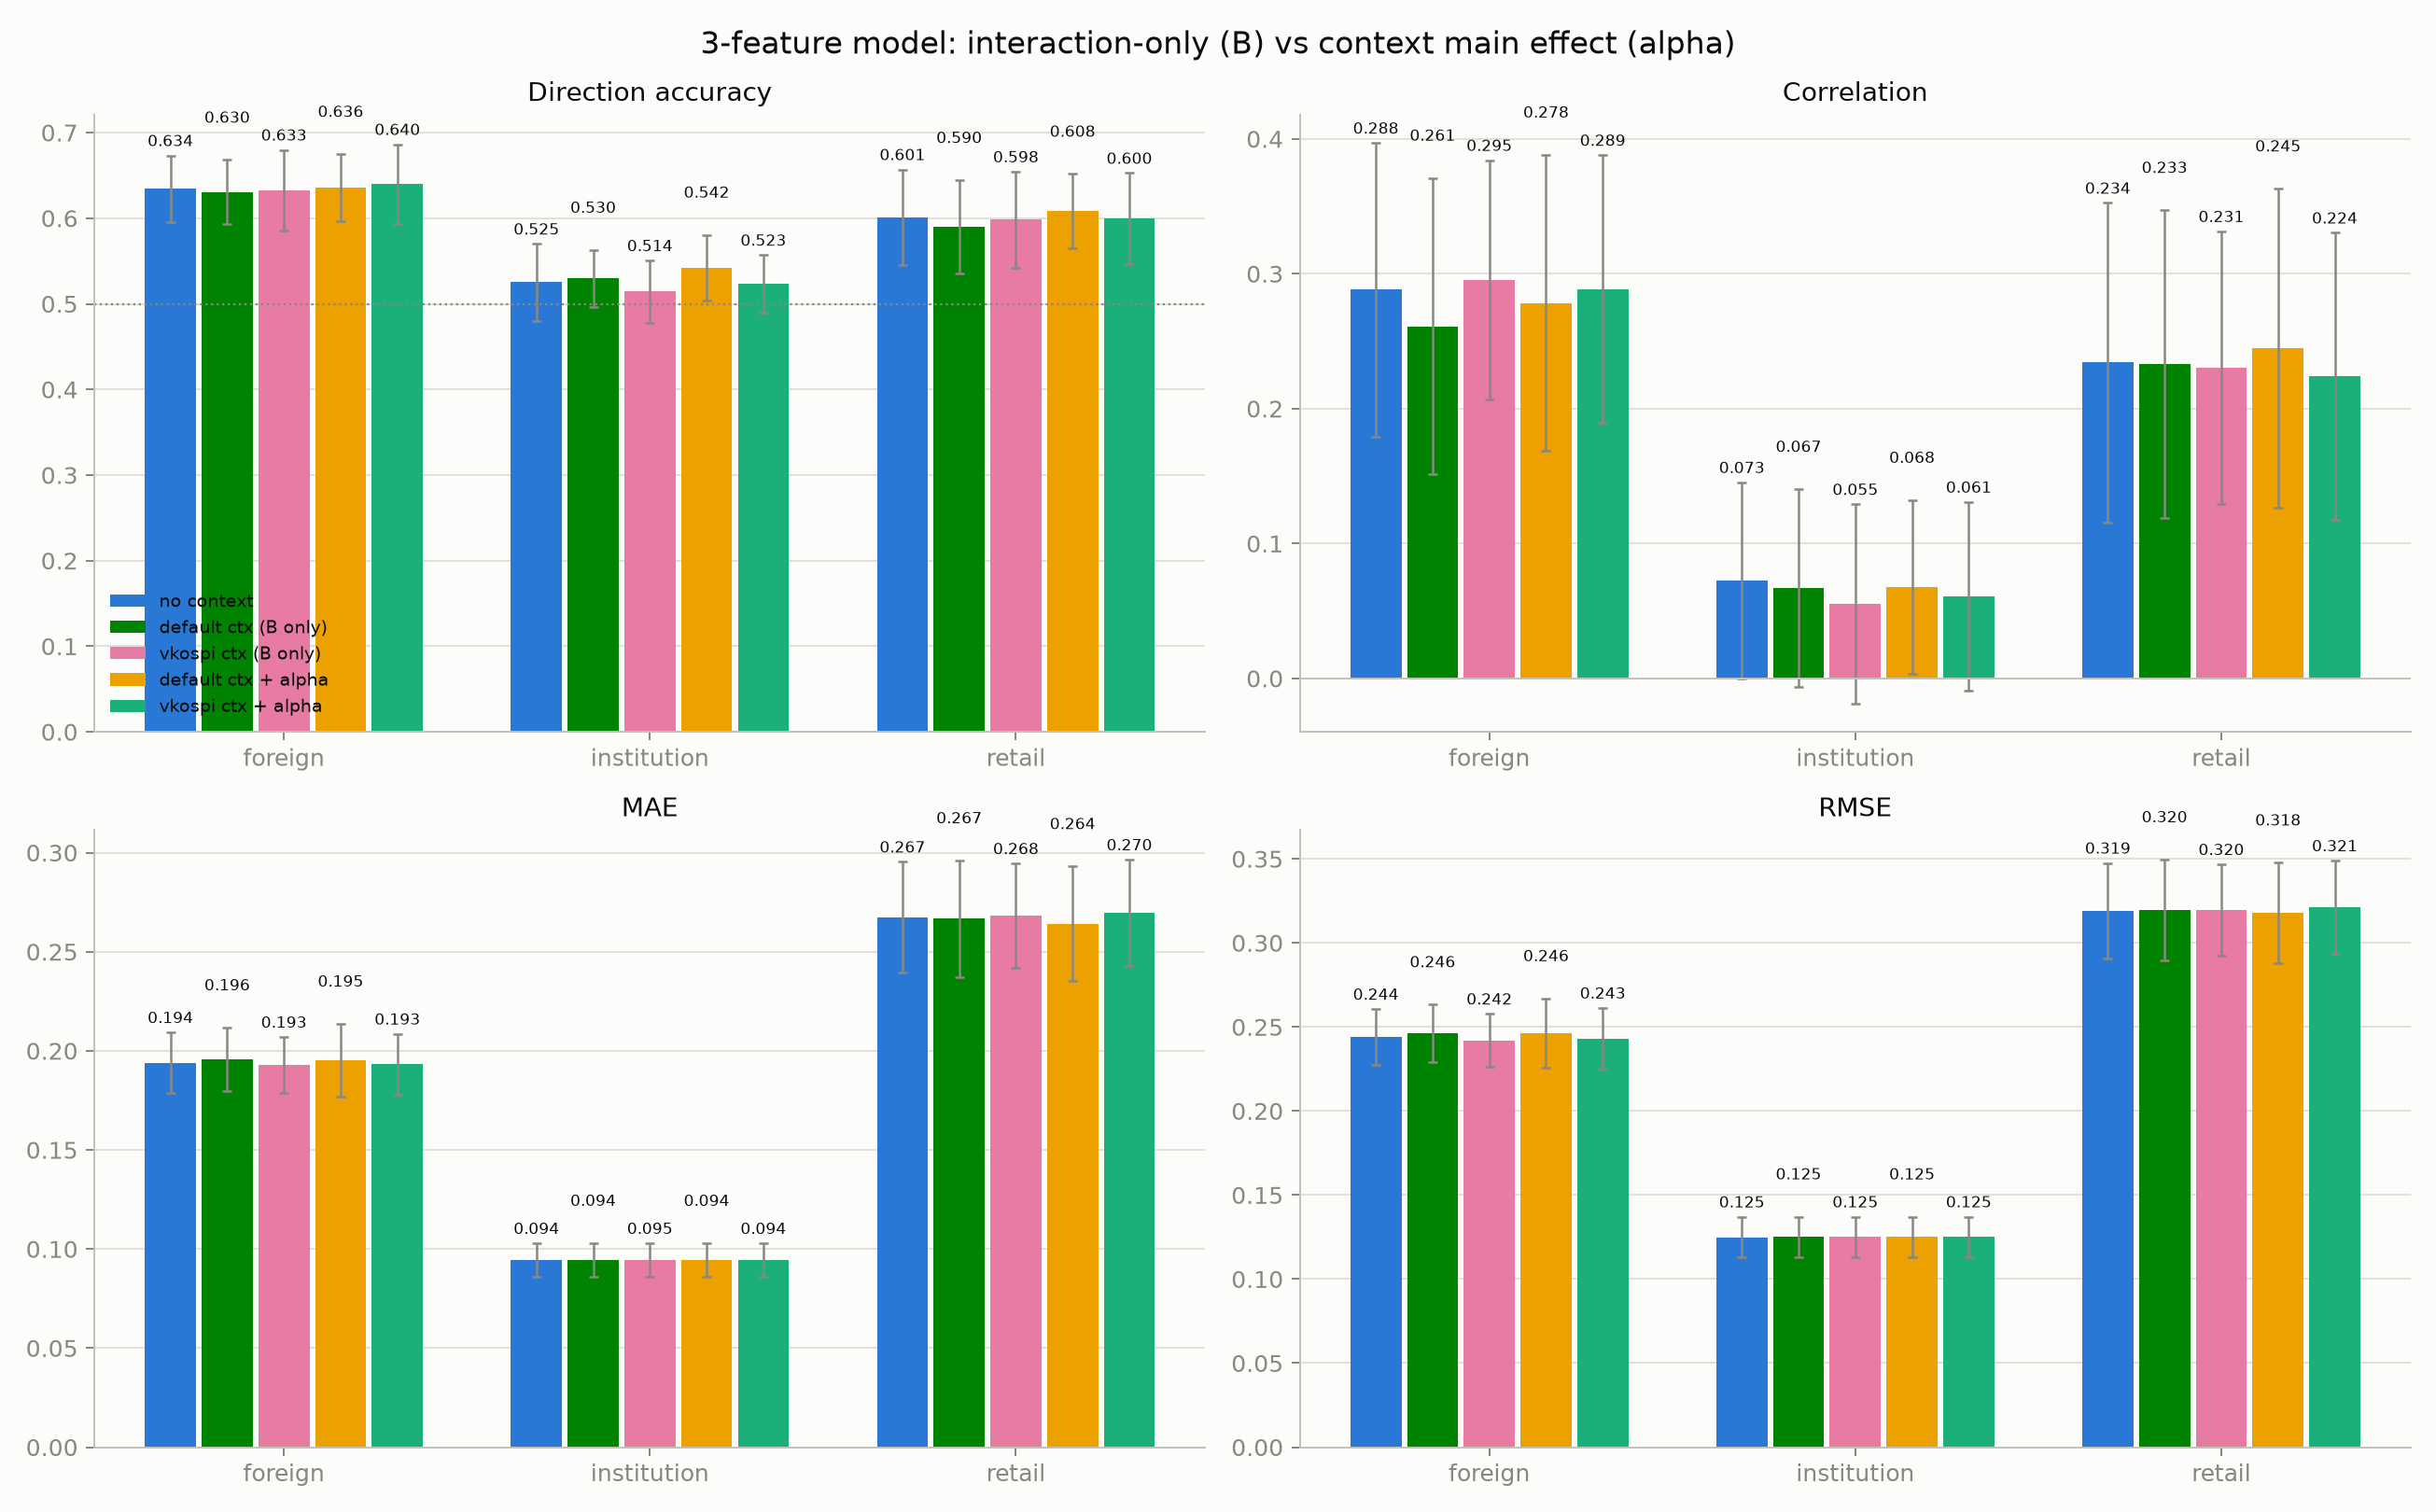
\includegraphics[width=\textwidth]{../experiments/2026-07-19/1658_continuous_reward3_ctxmain_graphs/comparison_ctxmain_oos.png}
  \caption{동일한 세 보상 특징에서 컨텍스트 없음, 상호작용 $B$만 사용,
  컨텍스트 주효과 $\alpha$ 포함 모형의 외표본 성능 비교. 막대와 오차선은 각각
  45개 CPCV 분할의 평균과 표준편차다. 본 논문의 주모형은
  \texttt{default ctx + alpha}이다.}
  \Description{외국인, 기관, 개인의 방향 정확도, 상관, MAE, RMSE를 다섯 개
  컨텍스트 변형에 대해 비교한 네 개의 막대그래프.}
  \label{fig:comparison}
\end{figure*}

다만 이 개선을 확정적 일반화 증거로 보기는 어렵다. 첫째, 모형 간 평균 차이는
대부분 각 모형의 분할 간 표준편차보다 작고, 겹치는 CPCV 시험표본 때문에 단순한
독립표본 검정도 적절하지 않다. 둘째, 현재 결과는 seed 42의 단일 학습 반복이며,
별도 미사용 기간의 순차 검증이나 다중 seed 재현은 수행되지 않았다. 셋째, 보상
가중치는 표준화된 관측 특징 사이의 조건부 연관을 나타내며 인과효과가 아니다.
넷째, 본 연구는 삼성전자 단일 종목의 집계 수급을 사용하므로 개별 계좌의 거래 목적,
보유기간, 주문 순서와 종목 간 일반화를 확인할 수 없다. 마지막으로 행동 재현
성능은 투자전략의 수익성과 다르며, 본 결과만으로 매매 규칙을 제시할 수 없다.

그럼에도 외국인과 개인의 반대 모멘텀, 공통적인 집단 간 반대매매, 개인의 양의
손실구간 계수, 그리고 서로 반대인 KOSPIㆍ환율 주효과는 하나의 단순한 모형 안에서
일관된 투자자 이질성을 보여 준다. 후속 연구에서는 (1) 여러 seed와 완전한
walk-forward 검증, (2) 다른 대형주와 시장 국면에 대한 외부 검증, (3) 컨텍스트
주효과만 있는 축소모형과의 ablation, (4) 계좌 수준 보유자료를 이용한 손실구간
특징 검증이 필요하다.

\bibliographystyle{ACM-Reference-Format}
\bibliography{paper-ko}

\end{document}
